Maps and paths will be visualized in form of web application. It should be accessible from internet and connect to specific system to fetch live data. Mock of the visualization is shown on the figure \ref{fig:vis_mock}. 

\begin{figure}[H]
    \centering
    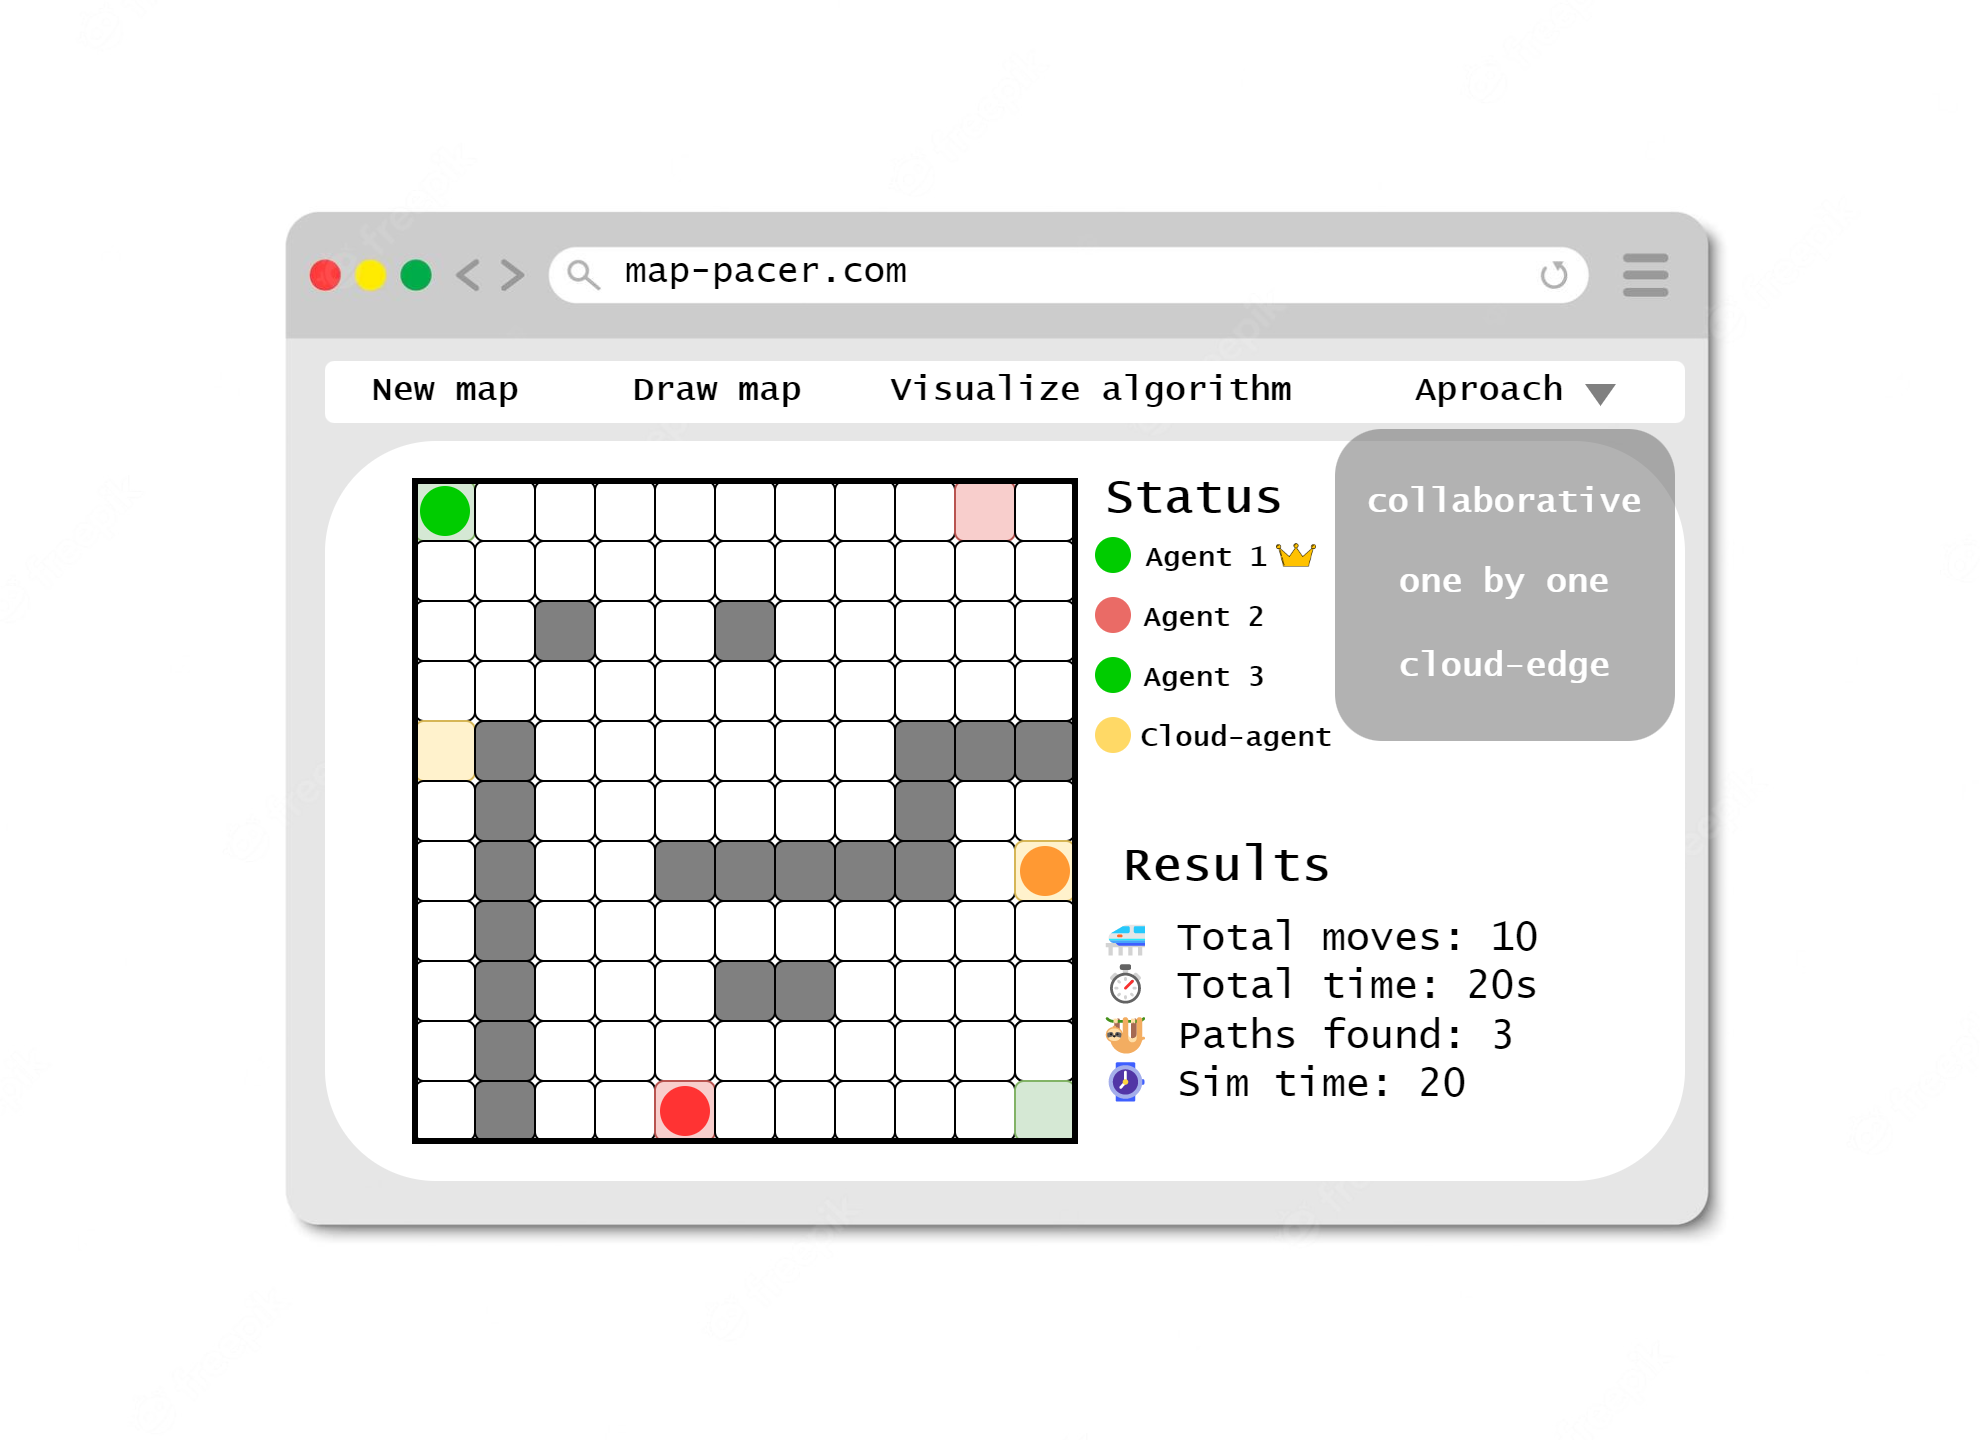
\includegraphics[width=\textwidth]{pictures/frontenf_mock.png}
    \caption{ Mock of the visualization }
    \label{fig:vis_mock}
\end{figure}

Graphical interface will be centered around gridmap which indicates positions and goal of all the agent(marked as coloured dots). On a side of the map will be status of the agent, indication of current leader and some details about result of the algorithm.

Through webapp, user will be able to(core functionality):
\begin{itemize}
\itemsep0em 
    \item Generate new map(random or predefined map)
    \item Create new map
    \item Select algorithm
    \item Visualize algorithm
\end{itemize}
Additional features:
\begin{itemize}
\itemsep0em 
    \item Access map creator, to specify own map.
    \item Choose among different systems(multi tenancy).
    \item Reply visualization.
\end{itemize}